\chapter{Didaktické príklady}

Pre AeroShield bolo v prostredí Arduino IDE, MATLAB a Simulink vytvorených niekoľko vzorových programov, ktoré demonštrujú všetky jeho funkcie a možnosti operácie. Programy sú rozdelené do dvoch veľkých skupín, konkrétne programy v otvorenej slučke bez spätnej väzby a programy v uzavretej slučke so spätnou väzbou. 

Ich rozdiel spočíva v tom že pri riadení bez spätnej väzby, hovoríme o ovládaní systému, kedy sa snažíme dosiahnuť žiadané hodnoty výstupov bez spätnej informácie o vykonaní procesu, alebo o jeho hodnote. V prípade riadenia so spätnou väzbou sa jedná o reguláciu. Pri regulácii sa kontroluje bezprostredný účinok riadenia, ktorý sa porovnáva so žiadanou hodnotou výstupu a na vyrovnanie ich vzájomnej chyby, sa okamžite vykonáva zásah do vstupných veličín. 

\section{Programy v otvorenej slučke, bez spätnej väzby}
\subsection{$AeroShieldOpenLoop.ino$}

Ako prvý príklad si ukážeme program s názvom \verb|AeroShield_OpenLoop.ino| napísaný v prostredí Arduino IDE. Hlavnou ideou tohoto programu je jednoduché ovládanie otáčok motorčeka kyvadla, pomocou potenciometra. Na začiatku programu inicializujeme hlavnú knižnicu AeroShieldu pomocou príkazu \verb|#include "AeroShield.h"|. Následne deklarujeme premenné, ktorých hodnoty budú vypisované na sériový monitor. 

\begin{lstlisting}[caption={AeroShield open loop dekleracia.},captionpos=b]
#include "AeroShield.h"       //  Inicializacia hlavnej kniznice

float startangle=0;           //  Premenna pre nulovy uhol
float lastangle=0;            //  Premenna pre maximalny uhol 
float pendulumAngle;          //  Uhol natocenia kyvadla
float referencePercent;       //  Hodnota potenciometra
float CurrentMean;	      //  Hodnota prudu odoberaneho motorom 
\end{lstlisting}

Nasleduje časť \verb|setup()|, v ktorej ako prvé, prebehne nastavenie rýchlosti sériovej komunikácie \verb|Serial.begin(115200)|. Číslo 115 200 predstavuje počet zmien, stavu z 0 na 1 resp. zo stavu high na stav low, za sekundu. Nasleduje funkcia \verb|AeroShield.begin()| ktorá sleduje prítomnosť magnetu, a pred nastaví potrebné premenné a funkcie pinov. Poslednou funkciou je kalibrácia kyvadla \verb|AeroShield.calibration()|, spolu s výpočtom začiatočného a koncového uhla. 

\begin{lstlisting}[caption={AeroShield open loop setup().},captionpos=b]
void setup() {                // Setup prebehne len jeden krat 
 Serial.begin(115200);       // Zaciatok seriovej komunikacie 
 AeroShield.begin(AeroShield.detectMagnet());  // Inicializacia AeroShieldu 
 startangle = AeroShield.calibration(AeroShield.getRawAngle());   // Kalibracia kyvadla
 lastangle=startangle+1024;  // Kalkulacia uhlu kyvadla pre map function
}
\end{lstlisting}

V časti \verb|loop()| sa program opakuje dookola. Ako prvé, prebehne mapovanie uhlu kyvadla pomocou funkcie \verb|AutomationShield.mapFloat()| a získaná hodnota uhlu sa vypíše na sériový monitor, spolu s názvom a premennou danej veličiny. Nasleduje čítanie hodnoty potenciometra, ktorá slúži na ovládanie akčného člena pomocou funkcie \verb|AeroShield.actuatorWrite()|. Na sériový port sa vypíše hodnota potenciometra obr.\ref{OBRAZOK 3.1}, za ktorou nasleduje veľkosť prúdu odoberaného motorom \verb| AeroShield.currentMeasure()|. 

\begin{lstlisting}[caption={AeroShield open loop loop().},captionpos=b]
void loop() {
	pendulumAngle= AutomationShield.mapFloat(AeroShield.getRawAngle(),startangle,lastangle,0.00,90.00);    //  Mapovanie uhlu kyvadla 
	Serial.print("pendulum angle is: ");
	Serial.print(pendulumAngle);    
	Serial.print("Degrees || ");
	
	referencePercent= AeroShield.referenceRead();  // Citanie potenciometra
	Serial.print("pot value is: ");
	Serial.print(referencePercent);  
	Serial.print("% || ");
	
	AeroShield.actuatorWrite(referencePercent); // Pohyb akcneho clenu
	
	CurrentMean= AeroShield.currentMeasure();  // Meranie prudu
	Serial.print("current value is: ");
	Serial.print(CurrentMean);   
	Serial.println("A || ");
}
\end{lstlisting}

\begin{figure}[!tbh]
	\centering
	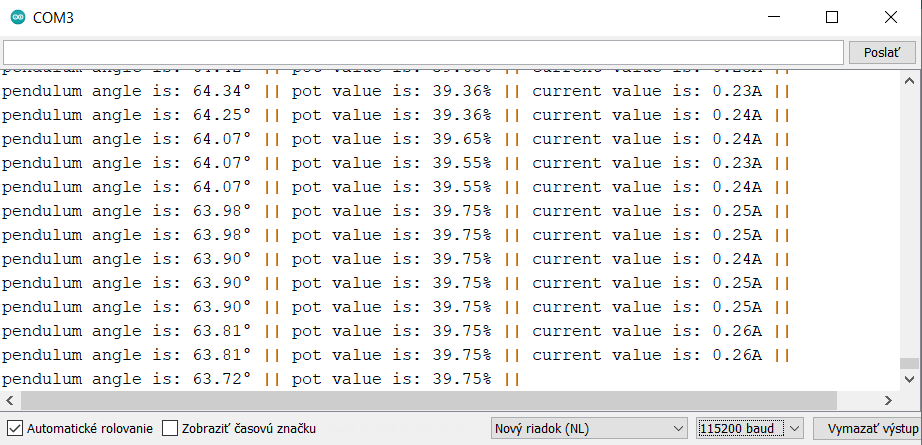
\includegraphics[width=120mm]{obr/VystupOLIDE.png}
	\caption{Výstup z programu AeroShieldOpenLoop.ino.}\label{OBRAZOK 3.1}
\end{figure}

\subsection{$AeroShieldOpenLoop.m$}

V príklade \verb|AeroShieldOpenLoop.m| si ukážeme výhody a možnosti zobrazovania výstupov, v prostredí MATLAB. Výstupy vieme zobrazovať nielen na sériovom monitore alebo zapisovači, ale máme možnosť tvoriť grafy, tabuľky... a všetky tieto výstupy upravovať a ukladať podľa vlastných predstáv a požiadaviek. 


Na začiatku kódu vymažeme všetky premenné a objekty, pomocou série príkazov \code{Clear all, clear a, clc}. Následne načítame knižnicu AeroShieldu a vykonáme funkciu \verb|AeroShield.begin()|. Nasleduje kalibrácia nulového uhlu kyvadla a zadefinovanie premenných na počítanie času, ako aj premenné na ukladanie hodnôt potenciometra a uhlu kyvadla. 

\begin{lstlisting}[caption={AeroShield open loop inicializacia.},captionpos=b]
% vymazanie premennych a objektov 
clear all;
clear a;
clc 

% nacitanie kniznice AeroShieldu  
AeroShield=AeroShield;
% vytvorenie objektov arduino, as5600
AeroShield.begin();
% kalibracia
startangle= AeroShield.calibration(); 
lastangle=startangle+2048; 

% premenne na pocitanie casu
time = 0;
count = 0;
angle = 0;          % uhol kyvadla
potentiometer = 0;  % hodnota potenciometra
\end{lstlisting}

Ďalej pokračujeme s definovaním vlastností grafu na zobrazovanie hodnôt potenciometra a uhlu kyvadla. Zvolili sme spôsob kontinuálneho vykresľovania grafu, kedy obe strany grafu zobrazujú rozdielne premenné a rozsahy, ktoré sa prispôsobujú veľkosti premenných. Zapisovanie premenných na rôzne strany grafu funguje vďaka príkazom, \verb|yyaxis right| a \verb|yyaxis left|, za ktorými nasleduje samotné vykreslenie grafu pomocou príkazu \verb|plot()|. Volíme si taktiež názvy osí grafu a jeho legendu. Medzi vykresleniami jednotlivých premenných použijeme príkaz \verb|hold on|, ktorý zabezpečí zapísanie premenných do jedného grafu. Na konci kódu je príkaz \verb|tic| ktorý začne počítať prejdený čas, od jeho spustenia. 

\begin{lstlisting}[caption={AeroShield open loop grafy.},captionpos=b]
	yyaxis right                      % set plotting to right axis 
	plotGraph = plot(time,angle,'-r' )      % plotting angle value
	ylabel('Angle (degree)','FontSize',15);      % label settings
	xlabel('Time (s)','FontSize',15);       % label settings
	hold on       % hold on makes sure all of the variables are plotted
	
	yyaxis left                             % Set plotting to left axis
	plotGraph1 = plot(time,potentiometer,'-b') % plotting potentiometer value
	title('Pendulum plot','FontSize',15);      % title settings   
	ylabel('Percent','FontSize',15)            % label settings
	legend('Potentiometer value','Pendulum angle')   % legend for plots
	grid('on');                      % grid for plot 'off' to turn off grid
	
	tic                              % time keeping
\end{lstlisting}

Nasleduje while cyklus ktorý má podmienku ukončenia zatvorenie vykresľovaného grafu tj. v momente kedy zatvoríme graf, podmienka prestane byť splnená a program sa ukončí. V cykle najskôr čítame hodnotu potenciometra pomocou \verb|AeroShield.referenceRead()| a túto hodnotu zapisujeme na akčný člen vďaka príkazu \verb| AeroShield.actuatorWrite()|. Nasleduje čítanie uhlu kyvadla \verb|AeroShield.getRawAngle()|, za ktorím prebehne mapovanie premennej z hodnoty raw na stupne. Premenná \verb|count| slúži na počítanie počtu prejdených cyklov, ako aj na tvorbu usporiadaného radu premenných, a využívame ju aj na vykresľovanie pohyblivej x-ovej osi grafu obr.\ref{OBRAZOK 3.2}. Ľavá stupnica grafu je stacionárna a zobrazuje hodnotu potenciometra, pravá stupnica zobrazuje uhol kyvadla v stupňoch a svoje rozpätie zväčšuje alebo zmenšuje v závislosti na výchylke kyvadla. Na konci programu ešte nájdeme if podmienku, ktorá kontroluje uhol kyvadla. Ak ten nadobudne hodnotu väčšiu ako 110°, proces sa automaticky ukončí a vypíše sa upozornenie. Posledný príkaz \verb|clear AeroShield.arduino| vymaže objekt \verb|arduino| a pripraví MATLAB na spustenie ďalšieho programu. 

\begin{lstlisting}[caption={AeroShield open loop, while cyklus.},captionpos=b]
while ishandle(plotGraph)           % loop will run until plot is closed
	
	pwm = AeroShield.referenceRead();   % read potentiometer value
	AeroShield.actuatorWrite(pwm);      % actuate 
	RAW= AeroShield.getRawAngle();      % read raw angle value
	angle_ = mapped(RAW, startangle, lastangle, 0, 180); % map raw value to degree 
	
	count = count + 1;                              % cycle counter
	time(count) = toc;                              % time keeping
	angle(count) = angle_(1);                       % angle value in time
	percenta= mapped(pwm, 0.0, 5.0, 0.0, 100.0);    % map pwm to percent 
	potentiometer(count) = percenta(1);             % pententiometer value in time
	set(plotGraph,'XData',time,'YData',angle);      % plot first data 
	set(plotGraph1,'XData',time,'YData',potentiometer); % plot second data 
	axis([time(count)-5 time(count) 0 100]);        % "running" x axis settings
	
	if (angle_ > 110)                            % if angle of pendulum bigger than 110degree
	AeroShield.actuatorWrite(0.0);      % stop the motor 
	disp('Angle of pendulum too high. AeroShield is turned off')
	break                               % stop the program
	end
end  

clear AeroShield.arduino;           
\end{lstlisting}

\begin{figure}[!tbh]
	\centering
	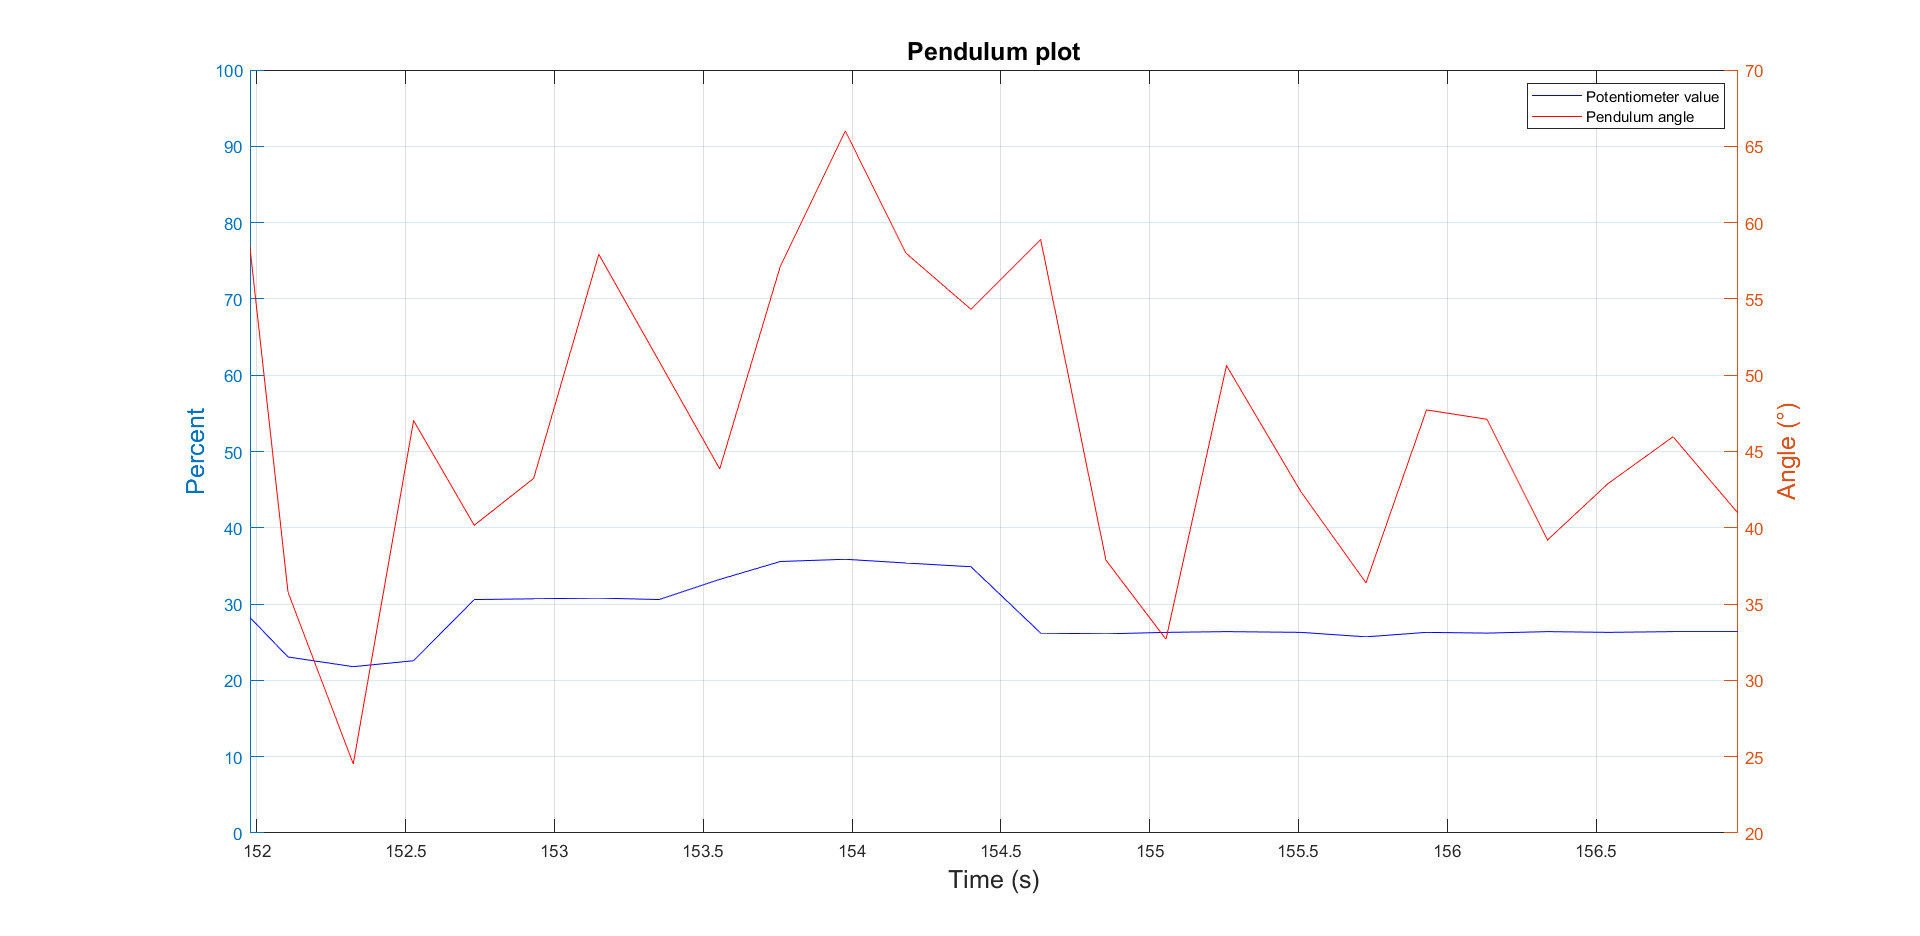
\includegraphics[width=\textwidth]{obr/ASOLmat.png}
	\caption{Výstup z programu AeroShieldOpenLoop.m.}\label{OBRAZOK 3.2}
\end{figure}

\section{Programy v uzatvorenej slučke, so spätnou väzbou}

sampling aj